\documentclass{article}

\usepackage{amsmath,amsthm}     
\usepackage{graphicx}     
\usepackage{hyperref} 
\usepackage{url}
\usepackage{amsfonts} 
\usepackage[margin=1in]{geometry}
\usepackage{float}
\usepackage{multicol, multirow}
\usepackage{arydshln}
\usepackage{subcaption}
\usepackage[french]{babel}
\usepackage{adjustbox}



\allowdisplaybreaks

\makeatletter
\@addtoreset{footnote}{page}
\makeatother

%%%%%%%%%%%%%%%%%%%%%%%%%%%%%%%%%%%%%%%%%%%%%%%%%%
\begin{document}

\renewcommand{\arraystretch}{1.5}

\title{BIML NLP : Classification d'émotions \\
\footnotesize{}}
\author{Bonhoure Timothé, Martinez Christophe}                      %%%% your final manuscript.

\maketitle
\tableofcontents
\section*{Introduction}
Ce projet a été réalisé par Timothé Bonhoure et Christophe Martinez. 
Il a été réalisé pour le cours de Bio-Inspired Machine Learning (BIML) du parcours Inteligence Artificielle du M2 Informatique à Lyon1
L'ensemble des fichiers de ce projet peuvent être trouvé à l'adresse \href{https://forge.univ-lyon1.fr/timothe.bonhoure/biml-nlp}{suivante}
\newpage

\section{Modèle}
\subsection{Architecture}
Notre architecture de modèle suit fidèlement les spécifications du sujet (voir Figure \ref{fig:modele_rnn}). Le processus commence par l'encodage en One Hot d'un mot en entrée, suivi d'un passage à travers une couche linéaire d'embedding. Par la suite, le modèle concatène la sortie de cette couche d'embedding avec des données cachées internes au modèle, permettant ainsi la mémorisation des mots précédents dans la phrase. Enfin, ces données sont traitées par deux couches en parallèle pour produire en sortie une classification de l'émotion associée à la phrase. De manière récurrente, les informations résultantes sont également réinjectées dans les données cachées pour le traitement du mot suivant. \\
Toutes les couches sont des couches linéaires dont nous initialisons les poids avec la méthode\\ \texttt{nn.init.xavier\_uniform\_} permettant d'après nos recherches d'atténuer les effets de vanishing et d'exploding du gradient.

\begin{figure}[H]
    \centering
    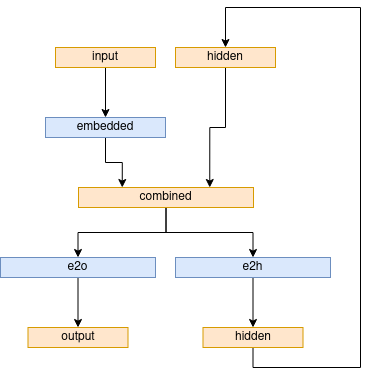
\includegraphics[width=0.4\linewidth]{img/modele.png}
    \caption{Modèle RNN}

    \label{fig:modele_rnn}
\end{figure}
\subsection{Entrainement}
La tâche principale de notre modèle consiste à classifier l'émotion associée à une phrase donnée. 
Pour entraîner notre modèle, nous avons choisi d'utiliser la fonction de perte \texttt{CrossEntropyLoss}. 
Cette fonction est largement adoptée dans les tâches de classification, en raison de sa capacité à inciter le modèle à être plus confiant dans ses prédictions. 
En effet, \texttt{CrossEntropyLoss} pénalise plus sévèrement les prédictions incorrectes associées à une forte confiance du modèle, favorisant ainsi une meilleure calibration des probabilités prédites. 

Pour optimiser notre modèle, nous avons opté pour l'utilisation de l'optimiseur \texttt{AdamW}. 
Cette variante améliorée de l'optimiseur \texttt{Adam} intègre une correction spécifique pour la régularisation des poids, résolvant ainsi le problème de dégradation du poids associé à l'optimiseur \texttt{Adam} standard. 

Lors de nos tests, nous avons observé une stabilisation de l'apprentissage au cours des 10 à 15 premières époques. 
Ainsi, choisir 20 époques pour réaliser l'entraînement complet de notre modèle nous est apparu comme un compromis judicieux entre la rapidité et la performance de l'apprentissage.
En ce qui concerne la taille du lot (\textit{batch size}), notre approche a été de la laisser non fixée et dépendante du cas de test spécifique. 
Nous avons adopté cette flexibilité pour nous adapter aux différentes situations d'expérimentation et ainsi évaluer la performance du modèle dans des contextes variés dans des temps comparables. 
Les valeurs de taille du lot varient entre 4 et 32 avec une valeur standard de 8.

Les classes d'émotions à prédire n'étant pas de taille similaire cela peu mener à un apprentissage concentré sur les classes les plus présentes au détriment de celles moins présentes.
Pour essayer de palier à ce problème, nous avons rajouté une pondération à \texttt{CrossEntropyLoss}.
Ces poids ont été prit inversement proportionnelle à la proportion de la classe dans l'ensemble des données.

\subsection{Fonctionnalités développées}
Dans ce modèle nous avons développé les fonctionnalités suivantes :
\begin{itemize}
    \item filtrage des mots rares
    \item filtrage des mots étant porteur de peu de sens (TF-IDF)
    \item apprentissage parallèle d'une tâche secondaire
    \item pondération des classes dans la loss
\end{itemize}


\section{Préparation des données}
Nous avons décidé de ne conserver que les mots dont la fréquence d’apparition est de minimum 5. 
Nous estimons que cela équivaut à retirer environ 77\% des mots de notre jeu de données, mais représente moins d'un mot par phrase.
L’effet de ce filtrage a pour effet d’accélérer grandement l’entraînement de notre modèle en réduisant grandement la taille de l'entrée. 

En analysant la distribution des longueurs de phrases dans notre ensemble d'entraînement, 
nous constatons une longueur moyenne d'environ 20 mots avec une variance de 120. 
Ces statistiques guident notre choix de définir une longueur maximale de phrases à 15 mots pour notre modèle. 

En plus de cela, nous recourons à la vectorisation TF-IDF pour chercher à extraire les caractéristiques de nos phrases en cherchant les mots les plus importants et significatifs. 
Parmi les 15 mots conservés de chaque phrase, nous avons préservé ceux présentant un meilleur score selon TF-IDF. 

Ainsi préparé, notre jeu de données est prêt à être utilisé dans l'entraînement de notre modèle de classification d'émotions. Cette préparation tient compte de la fréquence des mots, de la longueur des phrases, et des caractéristiques TF-IDF significatives, pour tendre au maximum vers une représentation riche et pertinente pour la classification.

\section{Tâche secondaire}
Une couche supplémentaire a été incorporée en parallèle (voir Figure \ref{fig:modele_rnn_with_secondary}) avec les deux précédentes pour accomplir une seconde tâche d'apprentissage basée sur la détection de la négation dans la phrase à classifier. 
Dans le cadre d'un prétraitement initial, les phrases ont été étiquetées comme étant négatives ou positives. 
Nous avons établi une liste de mots que nous considérons comme des indicateurs explicites de négation, notamment "not", "never", "neither", "no", "none", "nobody", "nowhere", et "nothing". 
Ainsi, toute phrase contenant au moins l'un de ces mots est étiquetée comme négative pour l'apprentissage de notre modèle. Pour la marque de négation en anglais "n't", la tâche d'étiquetage a été plus complexe. 
Pour des raisons de compatibilité des données, les apostrophes de "n't" ont été supprimées ("nt") et/ou remplacées par un caractère espace ("n t"). 
Ainsi, nous avons ajouté à la liste des indicateurs de négation le mot "t", mais il n'était malheureusement pas possible d'inclure tous les mots finissant par "nt" car cela englobe aussi des mots tels que "comment" et "radiant" qui ne sont pas des marqueurs de négation. 
Nous avons alors ajouté les mots "dont", "didnt", et "cant" qui sont les marqueurs suivant ce schéma les plus fréquents dans le jeu d'entraînement (entre 250 et 500 occurences). 

La tâche du modèle consiste désormais à prédire simultanément l'émotion associée à la phrase et à déterminer si la phrase est positive ou négative. Nous utilisons la fonction de perte \texttt{BCEWithLogitsLoss}, couramment utilisée pour la classification binaire. Dans notre cas, la classification de la phrase à travers cette tâche se résume à déterminer si la phrase est négative ou non. Ensuite, nous combinons cette perte avec la perte de la tâche principale en utilisant un poids préalablement défini afin d'évaluer une perte globale du modèle.

\begin{figure}[H]
    \centering
    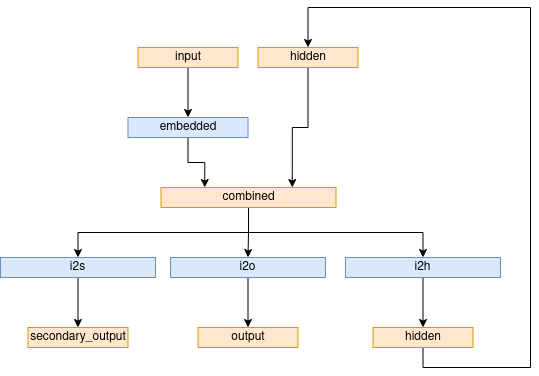
\includegraphics[width=0.5\linewidth]{img/modele_with_secondary.png}
    \caption{Modèle RNN avec tâche secondaire}

    \label{fig:modele_rnn_with_secondary}
\end{figure}

\section{Résultats}

\subsection{Modèle par défaut}
Notre modèle par défaut est entraîné sur 20 époques avec une taille de lots de 8, des tailles de couches (embedding et hidden) de 100, un taux d'apprentissage de $10^{-4}$, un poids de tâche secondaire de 0.1 et les fonctionnalités de filtrage des mots rares ou peu pertinents (TF-IDF, min\_freq) et de poids d'équilibrage des émotions (\textit{emotions\_weight}).
Pour estimer les capacités du modèle, nous avions tout d'abord commencé par calculer le score de précision du modèle.
Cependant, au vu du déséquilibre des classes, il nous a paru judicieux de s'appuyer sur un indicateur plus robuste aux inégalités entre les classes.
Nous avons décidé de prendre le coefficient de corrélation de matthews (aussi appelé \href{https://en.wikipedia.org/wiki/Phi_coefficient}{coefficient phi}) pour estimer les performances du modèle.

\begin{figure}[H]
    \centering
    \captionsetup{justification=centering}

    \adjustbox{center}{
        \begin{subfigure}{0.37\textwidth}
        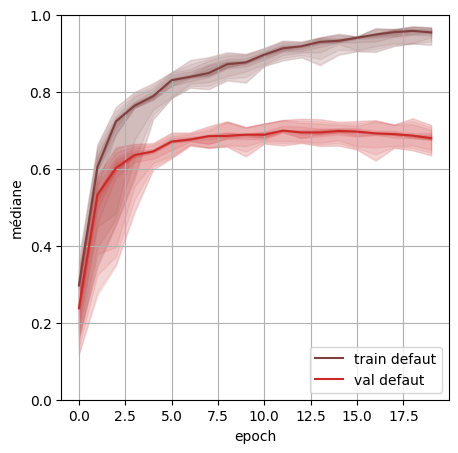
\includegraphics[width=\textwidth]{img/coefficient phi defaut median.png}
        \centering
        \caption{Coefficient phi }
        \end{subfigure}
        \begin{subfigure}{0.37\textwidth}
        \includegraphics[width=\textwidth]{img/précision defaut median.png}
        \centering
        \caption{Précision}
        \end{subfigure}
        \begin{subfigure}{0.46\textwidth}
            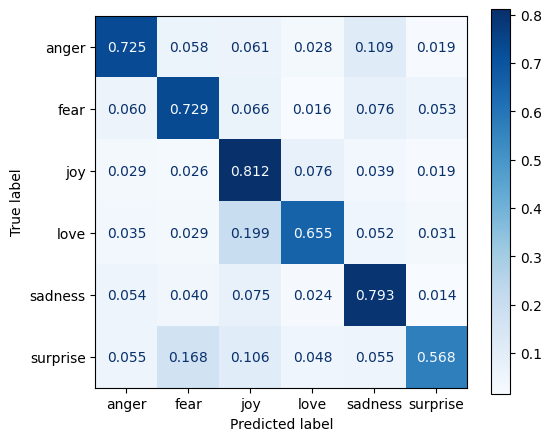
\includegraphics[width=\textwidth]{img/jeu de test defaut cm.png}
            \centering
            \caption{Matrice de confusion}
        \end{subfigure}
    }
    \caption{ Médiane et percentiles de la précision et du coefficient phi au cours de l'apprentissage}
\end{figure}

On remarque que les performances sur le jeu de validation arrive très vite à un plateau, voire ont tendance à redescendre sur les dernières epochs. Ainsi on voit qu'il était effectivement pas nécessaire de faire tourner le modèle sur plus d'epochs. 
On remarque de plus que la matrice de confusion est plutôt équilibré, mais que le modèle a du mal avec la classe "surprise" et confond pas mal les classes "joy" et "love"




Nous voulions savoir à quel point les fonctionnalités que nous avons implémentées pour la création de notre modèle permettait effectivement d'augmenter les performance de celui-ci.
Nous avons donc relancé le modèle en enlevant chacune de ces fonctionnalités une par une pour pouvoir voir leur effet séparé de tout autre variation.
\subsection{Modèle sans adaptation de la loss au déséquilibre des classes}
Nous avons ici enlevé les poids des classes.
Le but de cette fonctionnalité était de compenser le déséquilibre d'occurrence des classes en donnant un poids plus fort aux classes peu présente.
On s'attend donc peut être à une précision plus faible, mais à un coefficient phi plus élevé et à une matrice de confusion plus équilibré.
\begin{figure}[H]
    \centering
    \captionsetup{justification=centering}
    \begin{subfigure}{0.4\textwidth}
      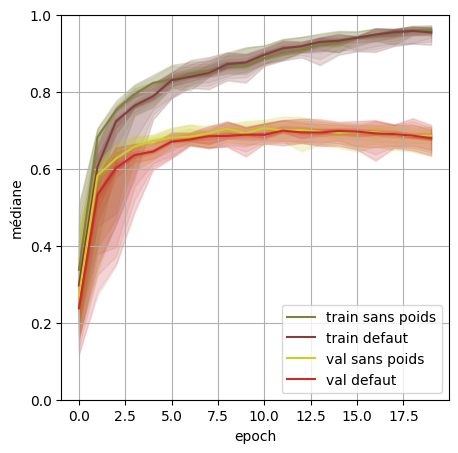
\includegraphics[width=\textwidth]{img/coefficient phi sans poids median.png}
      \centering
      \caption{Coefficient phi }
    \end{subfigure}
    \begin{subfigure}{0.4\textwidth}
      \includegraphics[width=\textwidth]{img/précision sans poids median.png}
      \centering
      \caption{Précision}
    \end{subfigure}
    \caption{
        Comparaison de la précision et du coefficient phi au cours de l'apprentissage\\
        entre avec et sans poids d'équilibrage
    }
    \label{fig:modele_sans_poids}
\end{figure}
Cependant, on se rend compte sur la figure \ref{fig:modele_sans_poids} qu'à la fois la précision et le coefficient phi sont légèrement inférieur avec les poids. 
En revanche, on remarque sur la figure \ref{fig:cm_sans_poids} que les poids permettent effectivement d'équilibrer la matrice de confusion.
En effet lest deux classes les moins présentes voit leur précision fortement augmenter (respectivement 10 et 15 pourcent). 
L'effet ne doit simplement pas être suffisant pour compenser la perte sur les classes les plus fréquentes (respectivement -5 et -3 pourcent) et ainsi donner un meilleur coefficient phi.

\begin{figure}[H]
    \centering
    \captionsetup{justification=centering}
    \begin{subfigure}{0.4\textwidth}
      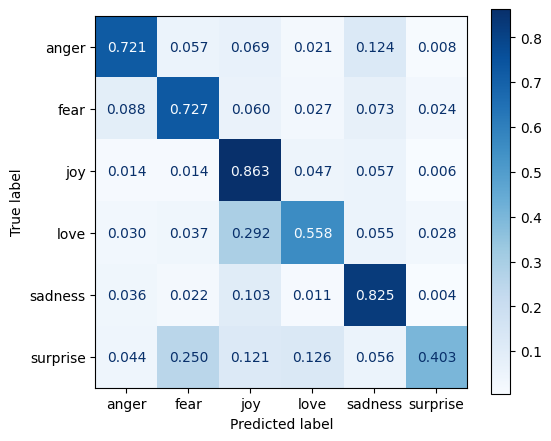
\includegraphics[width=\textwidth]{img/jeu de test sans poids cm.png}
      \centering
      \caption{Sans poids }
    \end{subfigure}
    \begin{subfigure}{0.4\textwidth}
      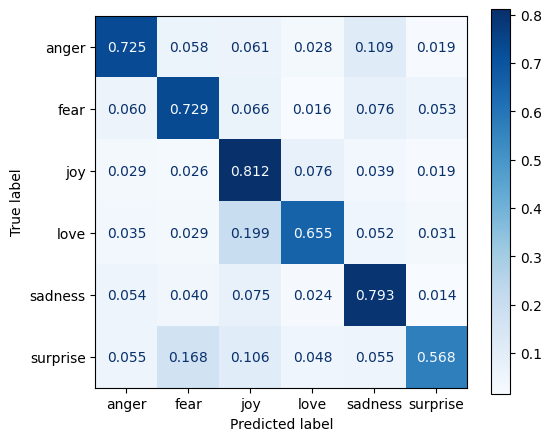
\includegraphics[width=\textwidth]{img/jeu de test defaut cm.png}
      \centering
      \caption{défaut}
    \end{subfigure}
    \caption{Comparaison des matrices de confusion entre avec et sans les poids d'équilibrage}
    \label{fig:cm_sans_poids}
\end{figure}



\subsection{Modèle sans tâche secondaire}
Nous avons ici enlevé l'apprentissage de la tâche secondaire.
Le but de cette fonctionnalité est de réduire le sur-apprentissage en augmentant la capacité de généralisation du modèle.
On s'attend donc à une performance supérieure sur le jeu de validation du modèle par défaut et une performance inférieur sur le jeu d’entraînement.
On remarque effectivement sur la figure \ref{fig:modele_sans_tache_sec} une faible tendance qui s'accentue au fur et à mesure que les epochs passe. Indiquant bien que la tâche secondaire aide à réduire le sur-apprentissage.

\begin{figure}[H]
    \centering
    \captionsetup{justification=centering}
    \begin{subfigure}{0.39\textwidth}
      \includegraphics[width=\textwidth]{img/coefficient phi sans tâche secondaire median.png}
      \centering
      \caption{Coefficient phi }
    \end{subfigure}
    \begin{subfigure}{0.39\textwidth}
      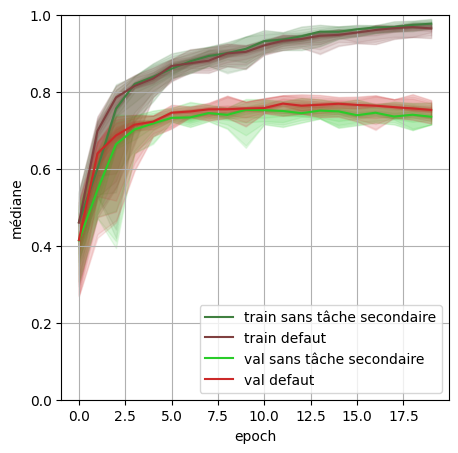
\includegraphics[width=\textwidth]{img/précision sans tâche secondaire median.png}
      \centering
      \caption{Précision}
    \end{subfigure}
    \caption{
        Comparaison de la précision et du coefficient phi au cours de l'apprentissage\\
        entre avec et sans apprentissage de la tâche secondaire
    }
    \label{fig:modele_sans_tache_sec}
\end{figure}
\subsection{Modèle sans TF-IDF}
Nous avons ici enlevé la sélection des mots les plus pertinents grâce à TF-IDF. 
Le but de cette fonctionnalité était de pouvoir concentrer un maximum d'information dans un minimum de mot.
On s'attend à avoir un effet positif sur la précision et le coefficient phi.
On remarque sur la figure \ref{fig:modele_sans_TF-IDF} que TF-IDF augmente sensiblement les performances du modèle.

\begin{figure}[H]
    \centering
    \captionsetup{justification=centering}
    \begin{subfigure}{0.39\textwidth}
      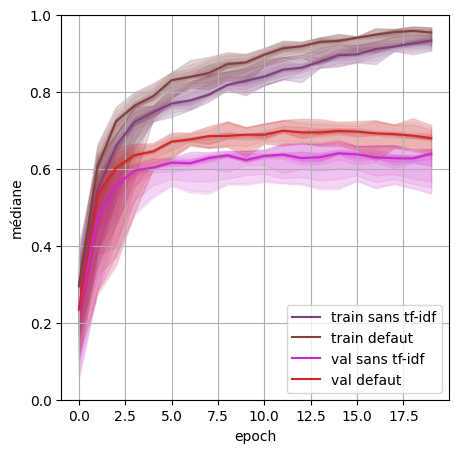
\includegraphics[width=\textwidth]{img/coefficient phi sans tf-idf median.png}
      \centering
      \caption{Coefficient phi }
    \end{subfigure}
    \begin{subfigure}{0.39\textwidth}
      \includegraphics[width=\textwidth]{img/précision sans tf-idf median.png}
      \centering
      \caption{Précision}
    \end{subfigure}
    \caption{
        Comparaison de la précision et du coefficient phi au cours de l'apprentissage\\
        entre avec et sans le filtrage avec TF-IDF
    }
    \label{fig:modele_sans_TF-IDF}
\end{figure}



\end{document}


